% Generated by experiments/make_appendix.py -- do not edit by hand.
% Every number is read from a committed run record at generation time.
% Requires: booktabs, amsmath, url, hyperref, graphicx.
% Labels are namespaced gen:* so they cannot collide with the
% author's own app:* appendix labels in the main file.

\section{Full per-cell results}
\label{gen:cells}

The main text reports a subset of cells. Both grids are given here in full, all twelve cells, as mean with a 95\% bootstrap confidence interval over 10 seeds. No row is omitted and no cell is excluded.

\subsection{Occurrence grid}

Run \texttt{20260830T002223Z\_6f98de3\_6e25cf7d}, git \texttt{6f98de3}, config \texttt{6e25cf7d}. 4000 sequences per seed, 3000 fit and 1000 held out, 20 models per cell differing only in initialization seed. A pair is \emph{indistinguishable} when a paired two-sided $t$-test on per-point held-out squared errors does not reject at $\alpha = 0.05$; all pooled statistics below are taken over indistinguishable pairs only.

\begin{table}[h]
\centering
\small
\begin{tabular}{llrlrrrr}
\toprule
width & depth & params & held-out $R^2$ & indist. & median $\rho$ & top-3 exact & top-3 Jaccard \\
\midrule
16 & 1 & 609 & 0.6011 \small[0.5725, 0.6274] & 162/190 & +0.917 & 26\% & 0.57 \\
16 & 2 & 881 & 0.5591 \small[0.5243, 0.5880] & 158/190 & +0.833 & 13\% & 0.43 \\
16 & 3 & 1,153 & 0.5349 \small[0.4948, 0.5677] & 134/190 & +0.817 & 9\% & 0.37 \\
32 & 1 & 1,217 & 0.6019 \small[0.5754, 0.6263] & 167/190 & +0.917 & 32\% & 0.62 \\
32 & 2 & 2,273 & 0.5537 \small[0.5110, 0.5909] & 143/190 & +0.817 & 12\% & 0.42 \\
32 & 3 & 3,329 & 0.4792 \small[0.4128, 0.5349] & 102/190 & +0.833 & 8\% & 0.36 \\
64 & 1 & 2,433 & 0.6278 \small[0.6003, 0.6544] & 160/190 & +0.933 & 48\% & 0.73 \\
64 & 2 & 6,593 & 0.5381 \small[0.4846, 0.5861] & 100/190 & +0.850 & 14\% & 0.43 \\
64 & 3 & 10,753 & 0.3929 \small[0.3309, 0.4483] & 92/190 & +0.900 & 6\% & 0.31 \\
128 & 1 & 4,865 & 0.6372 \small[0.6122, 0.6585] & 154/190 & +0.933 & 57\% & 0.78 \\
128 & 2 & 21,377 & 0.5836 \small[0.5369, 0.6259] & 144/190 & +0.883 & 27\% & 0.60 \\
128 & 3 & 37,889 & 0.4761 \small[0.3949, 0.5456] & 95/190 & +0.833 & 10\% & 0.38 \\
\bottomrule
\end{tabular}
\caption{Occurrence grid, all twelve cells. \emph{indist.} is the mean number of accuracy-indistinguishable pairs out of all pairs. \emph{median $\rho$} is the median per-instance Spearman correlation between the two models' per-position attribution magnitudes. \emph{top-3 exact} is the median over indistinguishable pairs of that pair's fraction of held-out sequences whose top-3 attributed sets match exactly, so it is a median over pairs of a per-pair fraction rather than a single pooled fraction over sequences.}
\end{table}

\subsection{Separation grid}

Run \texttt{20260830T030657Z\_972496a\_5da8cb38}, git \texttt{972496a}, config \texttt{5da8cb38}. Same library and split as above, sequence length 9. $Z$ is the number of held-out measurements needed to reject that a fit and its reparameterized twin are the same function, at $\alpha = 0.05$ with power 0.8, under the noise model of Appendix~\ref{gen:noise}.

\begin{table}[h]
\centering
\small
\begin{tabular}{llrllrr}
\toprule
width & depth & params & held-out $R^2$ & per-instance median $\rho$ & $Z$ to separate & top-3 exact \\
\midrule
16 & 1 & 609 & 0.984087 \small[0.979785, 0.987518] & 0.892 \small[0.877, 0.903] & 1 \small[0, 1] & 56\% \\
16 & 2 & 881 & 0.999241 \small[0.998708, 0.999619] & 0.978 \small[0.973, 0.983] & 42 \small[25, 60] & 82\% \\
16 & 3 & 1,153 & 0.999583 \small[0.999138, 0.999916] & 0.984 \small[0.978, 0.990] & 313 \small[87, 571] & 86\% \\
32 & 1 & 1,217 & 0.992155 \small[0.990567, 0.993674] & 0.872 \small[0.847, 0.893] & 0 \small[0, 1] & 48\% \\
32 & 2 & 2,273 & 0.997328 \small[0.995451, 0.999059] & 0.915 \small[0.892, 0.937] & 87 \small[14, 193] & 61\% \\
32 & 3 & 3,329 & 0.999166 \small[0.998775, 0.999529] & 0.923 \small[0.898, 0.945] & 833 \small[18, 2,136] & 61\% \\
64 & 1 & 2,433 & 0.998324 \small[0.997555, 0.998958] & 0.899 \small[0.886, 0.913] & 2 \small[1, 3] & 53\% \\
64 & 2 & 6,593 & 0.999997 \small[0.999995, 0.999998] & 0.855 \small[0.832, 0.880] & 4,176 \small[1,320, 7,333] & 48\% \\
64 & 3 & 10,753 & 0.999996 \small[0.999993, 0.999998] & 0.847 \small[0.835, 0.860] & 7,300 \small[2,156, 14,436] & 43\% \\
128 & 1 & 4,865 & 0.999876 \small[0.999862, 0.999889] & 0.923 \small[0.913, 0.933] & 9 \small[7, 11] & 54\% \\
128 & 2 & 21,377 & 1.000000 \small[1.000000, 1.000000] & 0.905 \small[0.888, 0.920] & 3,158,529 \small[1,402,633, 5,004,083] & 54\% \\
128 & 3 & 37,889 & 1.000000 \small[1.000000, 1.000000] & 0.890 \small[0.885, 0.895] & 87,751,464 \small[39,140,215, 138,392,840] & 53\% \\
\bottomrule
\end{tabular}
\caption{Separation grid, all twelve cells. $Z$ is a lower bound: it counts sequencing noise only (Appendix~\ref{gen:noise}).}
\end{table}

\begin{figure}[h]
\centering
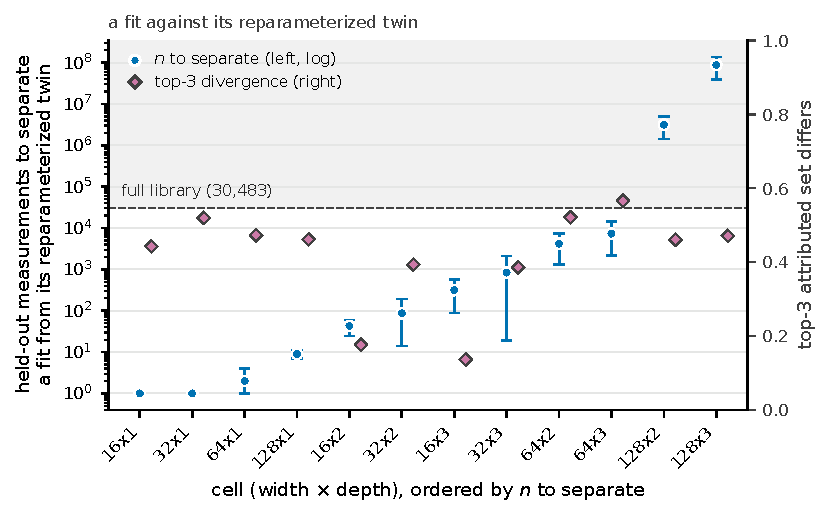
\includegraphics[width=0.85\linewidth]{figures/figA_twin_separability.pdf}
\caption{Separability and top-3 divergence for \textbf{a fit against its own reparameterized twin} --- \emph{not} for independently trained pairs. This is the separation experiment of the table above, and it is a different population from the one the main text figures describe: there, two models are trained independently and filtered to those the held-out data cannot tell apart; here, one fit is compared against a construction of itself. The two populations disagree substantially about how often the top-3 attributed set differs, so the numbers are not interchangeable and neither figure should be read as evidence for the other. Left axis logarithmic, spanning nine decades; the dashed line is the full library.}
\label{gen:twin}
\end{figure}

\section{Protocol}
\label{gen:protocol}

\paragraph{Split rule.}
Every experiment uses the same seeded split. For seed $k$, a \texttt{torch.Generator} is seeded with $1{,}000{,}003 + k$ and \texttt{torch.randperm}$(n)$ is drawn; the first 3000 indices are the fit split and the remaining 1000 are held out, from $n = 4000$ sequences. The split is therefore a deterministic function of the seed, identical across cells and across architectures within a seed, and the held-out indices are written into the run directory. Held-out points contribute nothing to any gradient.

\paragraph{Learning-rate ladder and selection.}
The ladder is learning rate over [0.01, 0.003, 0.001, 0.0003], selected once per cell and shared by all models in it. In the occurrence grid, ``no model selection: every trained model is kept and enters the pairwise analysis''. In the separation grid, ``pilot on the fit split's training loss''. The distinction matters for reading the two grids: the occurrence analysis is pairwise over all trained models, so discarding any model would bias the pair population it measures.

\paragraph{Epoch budget and seeds.}
Every cell in both grids is trained for 1,200 epochs (1,200 full-batch gradient steps), identical across width and depth so that capacity rather than budget separates the cells. Both grids use 10 seeds (0, 1, 2, 3, 4, 5, 6, 7, 8, 9), and every reported number is a mean over those seeds with a 95\% bootstrap confidence interval.

\paragraph{Tuning budget actually spent.}
Read from \texttt{tuning\_budget.json} in each run directory. The occurrence run records 12 entries, 4 configurations each, 48 configurations in total; the separation run records 12 entries, 4 each, 48 in total. The search space is the learning-rate ladder alone: no architecture, optimizer, initialization or budget search was performed, and no baseline received a larger budget than the method.

\paragraph{Configuration.}
The full resolved configuration is committed as \texttt{config.yaml} inside each run directory, alongside an \texttt{environment.lock} recording the interpreter and package versions the run actually used.

\section{Noise model derivation}
\label{gen:noise}

$Z$ requires an observation-noise scale. This library supplies one rather than needing an assumption, and the derivation is given here because the choice of count model changes $Z$ by orders of magnitude.

\paragraph{The phenotype is affine in a log count ratio.}
Each sequence carries two count pools, $\mathrm{ex}$ and $\mathrm{tot}$. Regressing the phenotype $y$ on $\log_{10}(\mathrm{ex}/\mathrm{tot})$ over the full library gives slope $0.9331$ $[0.9314, 0.9345]$ across seeds, and $r = 0.990$ over the full $30{,}483$-sequence library. The relationship is tight enough that the count ratio, not the phenotype, is the quantity whose noise must be modelled.

\paragraph{Why Poisson and not binomial.}
The two pools are \emph{not} numerator and denominator of a proportion. Over the committed library, $\mathrm{ex}$ exceeds $\mathrm{tot}$ in $4.9\%$ of rows, with ratios as large as $20.9$, and $\mathrm{ex} = 0$ in $11.4\%$ of rows. A binomial model is therefore not merely inefficient but undefined on roughly one row in twenty: $p = \mathrm{ex}/\mathrm{tot} \ge 1$ there, so the binomial variance $p(1-p)/\mathrm{tot}$ is zero or negative.

\paragraph{Delta method.}
Treating both pools as independent Poisson variates and applying the delta method to the log of their ratio,
\begin{equation}
\operatorname{var}\!\left(\log_{10} R\right) = \frac{1}{\ln(10)^2}\left(\frac{1}{\mathrm{ex}} + \frac{1}{\mathrm{tot}}\right),
\qquad
\mathrm{sd}(y_i) = |a|\,\frac{\sqrt{1/\mathrm{ex}_i + 1/\mathrm{tot}_i}}{\ln 10},
\end{equation}
with $a$ the fitted slope and a half-count continuity correction applied to both pools, which also covers the rows with $\mathrm{ex} = 0$. In the standardized units the models see, the median of this quantity is $0.3114$ $[0.3051, 0.3194]$.

\paragraph{The diagnostic that surfaced the binomial failure.}
The separation test weights points by $1/\sigma_i^2$, so a point assigned near-zero noise dominates the statistic. Under a binomial model a near-saturated sequence receives exactly that. The symptom was a weight distribution with a mean far above its median and a required sample size that collapsed to zero for every cell --- an implausible answer that is what prompted the check. Under the committed Poisson log-ratio model the mean of $1/\sigma^2$ is $3.0$ times its median, a heavy but unremarkable tail, and $Z$ becomes finite and cell-dependent. An unexamined count model would have reported that no data at all is needed to separate the fits.

We deliberately do not quote a magnitude for the binomial inflation. That model was replaced before the first commit of the separation experiment, so its exact variance form is not in the repository and the figure cannot be regenerated from committed code. What \emph{is} reproducible from the committed library is the structural defect above --- $p \ge 1$ on $4.9\%$ of rows, hence zero or negative binomial variance --- together with the Poisson ratio of $3.0$. Both were re-derived from the committed $30{,}483$-row library while preparing this appendix and agree with the recorded values.

\paragraph{$Z$ is a lower bound.}
This models sequencing noise only. Library preparation and biological variation add more, so the true noise is larger and the required sample size larger still. Every $Z$ in this paper should be read as ``at least this many''.

\section{The vacuous ceiling, in full}
\label{gen:ceiling}

\paragraph{The defect.}
The held-out closure experiment (run \texttt{20260829T181937Z\_b2951ae\_9fdd4067}, git \texttt{b2951ae}) reported that no cell contains the reparameterized twin, on the strength of a ceiling control that does not do the work it appears to do. Its refit path, \texttt{closure\_heldout.refit\_on\_split}, loads the reference weights, then evaluates the loss and snapshots the best iterate \emph{before} entering the optimisation loop. For the null target --- which is the reference's own latent --- the refit therefore begins at the answer. The measured initial loss is $6.7 \times 10^{-19}$, already below the $10^{-10}$ early-stop tolerance, so the loop breaks on its first iteration and returns the reference unchanged.

A held-out $R^2$ of $1.000000$ on that target is arithmetic, not evidence. It establishes that Adam does not wander away from a perfect solution. It does not establish that the refit can \emph{find} a solution it does not start at, which is the capability the containment conclusion depends on. Best-iterate selection is what makes the failure silent: because the initial state is already the best iterate ever seen, no subsequent step can displace it, and the procedure reports a perfect score without having searched.

\paragraph{The control that replaced it.}
Run \texttt{20260829T191427Z\_94dd5a2\_2267b74e}, git \texttt{94dd5a2}, config \texttt{2267b74e}, 10 seeds. The null target is refit \emph{without} warm-starting from the reference, from a cold random initialization. The target is known to be in the class, since the reference realises it, so this asks only whether the optimiser can travel to it. Mean initial loss across cells confirms the refit no longer begins at the answer.

\begin{table}[h]
\centering
\small
\begin{tabular}{llll}
\toprule
width & depth & cold-start null, held-out $R^2$ & warm warp refit, held-out $R^2$ \\
\midrule
16 & 1 & 0.9988 \small[0.9982, 0.9993] & 0.9748 \small[0.9669, 0.9809] \\
16 & 2 & 0.9476 \small[0.9244, 0.9703] & 0.9935 \small[0.9895, 0.9962] \\
16 & 3 & 0.7763 \small[0.6820, 0.8589] & 0.9959 \small[0.9921, 0.9986] \\
32 & 1 & 0.9994 \small[0.9990, 0.9997] & 0.9749 \small[0.9708, 0.9789] \\
32 & 2 & 0.8258 \small[0.7303, 0.9103] & 0.9463 \small[0.9185, 0.9724] \\
32 & 3 & 0.5626 \small[0.4404, 0.6891] & 0.9404 \small[0.9151, 0.9643] \\
64 & 1 & 0.9971 \small[0.9955, 0.9984] & 0.9804 \small[0.9696, 0.9893] \\
64 & 2 & 0.7122 \small[0.5620, 0.8561] & 0.9236 \small[0.8929, 0.9532] \\
64 & 3 & 0.4501 \small[0.3529, 0.5575] & 0.9034 \small[0.8879, 0.9186] \\
128 & 1 & 0.9969 \small[0.9962, 0.9975] & 0.9885 \small[0.9868, 0.9900] \\
128 & 2 & 0.8997 \small[0.8316, 0.9529] & 0.9575 \small[0.9381, 0.9734] \\
128 & 3 & 0.5328 \small[0.4000, 0.6714] & 0.9247 \small[0.9108, 0.9394] \\
\bottomrule
\end{tabular}
\caption{The ceiling that requires search. The cold-start column is an upper bound on what this procedure can say about any target, because its target is in the class by construction. Mean cold-start initial loss ranges from $1.826$ to $2.093$, against $6.7 \times 10^{-19}$ for the warm-started control it replaces.}
\end{table}

\paragraph{What the control shows.}
Read by depth: at depth 1 the worst-cell cold-start null reaches $0.9969$ against $0.9748$ for the warm warp refit, so the ceiling sits above the measurement; at depth 2 the worst-cell cold-start null reaches $0.7122$ against $0.9236$ for the warm warp refit, so the ceiling sits below the measurement; at depth 3 the worst-cell cold-start null reaches $0.4501$ against $0.9034$ for the warm warp refit, so the ceiling sits below the measurement.

At depth 1 the ceiling sits above the measurement, so the comparison is valid there and the warp target is genuinely not reached as well as an in-class one. At depths 2 and 3 the ranking inverts: the warm-started warp refit scores \emph{higher} than a cold-started refit to a target guaranteed to be in the class. That is initialization dominating the result, and no conclusion about what the class contains can be drawn at those depths. The configured pass threshold is $0.999$, and 11 of 12 cells fall below it.

The honest reading is therefore narrower than the original claim: the refit procedure did not find a member of the class equal to the twin. That is consistent with no such member existing, and equally consistent with one existing that the optimiser failed to reach.

\section{Reproducibility}
\label{gen:repro}

\paragraph{Repository.}
\url{https://github.com/shadi97kh/CERTGNN}. Every experiment writes a directory under \texttt{results/runs/} named \texttt{<timestamp>\_<gitsha>\_<confighash>}, containing the resolved \texttt{config.yaml}, an \texttt{environment.lock}, a \texttt{meta.json} recording the git SHA and whether the tree was dirty, a \texttt{tuning\_budget.json}, per-seed JSON, and the aggregated \texttt{results.json}. Every number in this paper is read from one of those files by a generator script; none is transcribed by hand.

\begin{table}[h]
\centering
\small
\begin{tabular}{lllll}
\toprule
experiment & run directory & git SHA & config hash & seeds \\
\midrule
\texttt{closure\_heldout} & \texttt{\scriptsize 20260829T181937Z\_b2951ae\_9fdd4067} & \texttt{b2951ae} & \texttt{9fdd4067} & 10 \\
\texttt{closure\_search} & \texttt{\scriptsize 20260829T191427Z\_94dd5a2\_2267b74e} & \texttt{94dd5a2} & \texttt{2267b74e} & 10 \\
\texttt{occurrence} & \texttt{\scriptsize 20260830T002223Z\_6f98de3\_6e25cf7d} & \texttt{6f98de3} & \texttt{6e25cf7d} & 10 \\
\texttt{separation} & \texttt{\scriptsize 20260830T030657Z\_972496a\_5da8cb38} & \texttt{972496a} & \texttt{5da8cb38} & 10 \\
\bottomrule
\end{tabular}
\caption{Every run directory cited in this paper. A run recorded against a dirty tree is marked; none of the runs cited here is.}
\end{table}

\paragraph{Pre-registration.}
\texttt{PREREGISTRATION.md} records the claims, the gate thresholds and the falsification conditions. It was committed on 2026-08-26 in \texttt{6d0719a} and has never been amended: its git history contains 1 commit. The earliest committed run directory dates from 2026-08-29, so the pre-registration predates every result reported here, and this is checkable from the repository history rather than asserted.

Amendment is additionally blocked by a tool-level pre-write hook, \texttt{scripts/hooks/protect\_prereg.sh}, registered as a \texttt{PreToolUse} hook. The hook matches the \emph{target path} of a write and refuses any edit whose destination is \texttt{PREREGISTRATION.md}, including shell redirections, \texttt{sed -i}, \texttt{mv}, \texttt{cp} and \texttt{rm} aimed at it. It deliberately does not fire on files that merely mention the pre-registration by name, an earlier behaviour that produced false positives and trained bypasses. The guard is inert until results exist, so the first write is permitted and every subsequent one is not. We state the mechanism precisely because it is a hook in the authoring environment rather than a server-side or \texttt{pre-commit} enforcement: it constrains the workflow that produced this paper, and the durable evidence is the single-commit git history above.
